\documentclass[conference,compsoc]{IEEEtran}
\usepackage{hyperref}

\usepackage[justification=raggedright,format=hang]{caption}

\usepackage{url}
\makeatletter
\g@addto@macro{\UrlBreaks}{\UrlOrds}
\makeatother

\usepackage{cite}
\usepackage{amsmath,amssymb,amsfonts}
\usepackage{algorithmic}
\usepackage{graphicx}
\usepackage{textcomp}
\usepackage{float}
\usepackage{xcolor}
\def\BibTeX{{\rm B\kern-.05em{\sc i\kern-.025em b}\kern-.08em
    T\kern-.1667em\lower.7ex\hbox{E}\kern-.125emX}}
    
\usepackage{epigraph}
\usepackage{listings}
\usepackage{adjustbox}
\usepackage{multirow}
\usepackage{array}
\usepackage{authblk}
\usepackage[ruled,vlined]{algorithm2e}

\newcommand{\myparagraph}[1]{\smallskip\noindent{\bf #1.}}
\newcommand{\myfirstparagraph}[1]{\noindent{\bf #1.}}
\newcommand{\scedit}[1]{{\color{black} #1}} % blue
    
\begin{document}

\title{FuzzSplore: Visualizing Feedback-Driven Fuzzing Techniques}

\iffalse
\author{\IEEEauthorblockN{Andrea Fioraldi}
\IEEEauthorblockA{\textit{1692419}}
\and
\IEEEauthorblockN{Luigi Paolo Pileggi}
\IEEEauthorblockA{\textit{1691249}}
}

\author{\IEEEauthorblockN{Andrea Fioraldi\IEEEauthorrefmark{1}\IEEEauthorrefmark{2},
Luigi Paolo Pileggi\IEEEauthorrefmark{1}}
\IEEEauthorblockA{andreafioraldi@gmail.com,
gigimail@gigi.com\\
\IEEEauthorrefmark{1} Sapienza University of Rome,
\IEEEauthorrefmark{2} EURECOM}}
\fi

\author[1]{Andrea Fioraldi}
\author[1]{Luigi Paolo Pileggi}
\affil[1]{Sapienza University, Rome, Italy \authorcr {\tt \{fioraldi.1692419, pileggi.1691249\}@studenti.uniroma1.it}\vspace{1.5ex}}

\maketitle

\begin{figure*}[t]
\centering
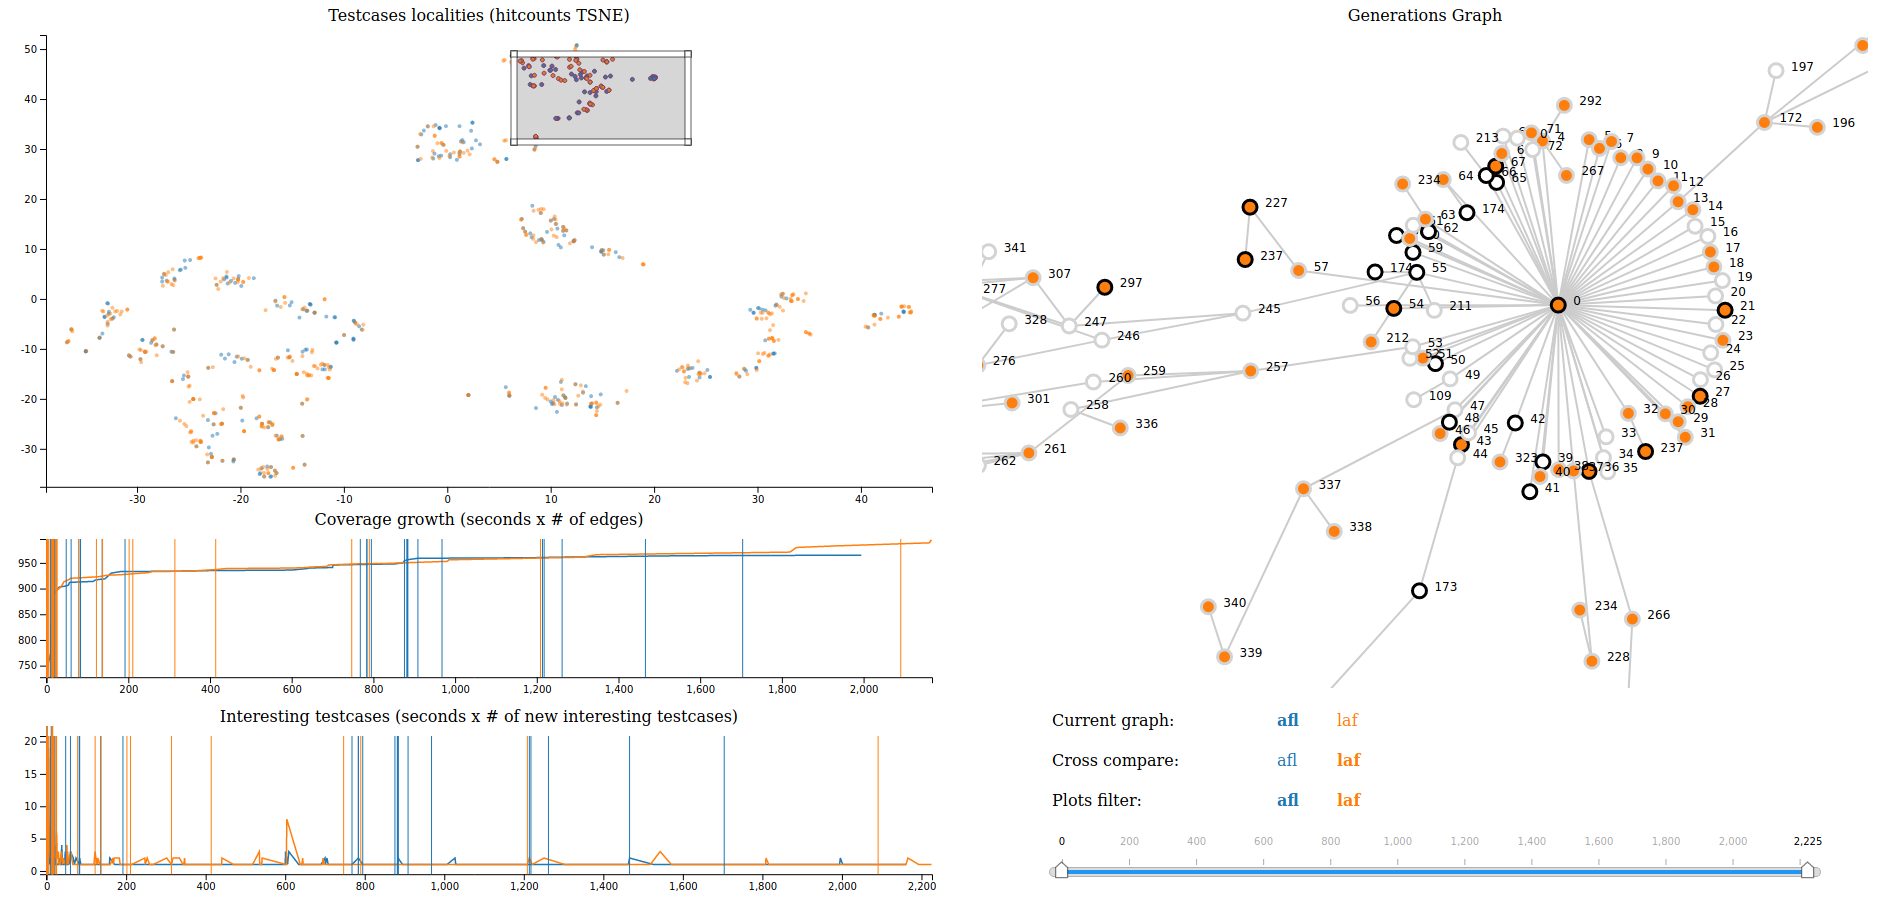
\includegraphics[width=1.0\textwidth]{img/full}
\caption{Complete view of the {\sc FuzzSplore} visual panel.}
\label{fig:full}
\end{figure*}

\begin{abstract}
Fuzz Testing techniques are the state of the art in software testing for security issues nowadays.
Their great effectiveness attracted the attention of researchers and hackers and involved them in developing a lot of new techniques to improve Fuzz Testing.
The evaluation and the cross-comparison of these technique is an almost open problem. In this paper we propose a human-driven approach to this problem based on information visualization.
We developed a prototype upon the {\sc AFL++} fuzzing framework, {\sc FuzzSplore}, that an analyst can use to get useful insights about different fuzzing configurations applied to a specific target in order to choose or tune the best technique during a fuzzing campaign.
\end{abstract}

\section{Introduction}

{\em Fuzz Testing} or {\em Fuzzing} is a family of techniques to automatically uncovers bugs in software.

Due to its effectiveness, much more efficient than other software testing techniques like {\it Symbolic Execution} \cite{redqueen} \cite{sebastian}, the research in this field is flourishing and several different techniques were developed to improve fuzz testing, both from academy and industry.

The evaluation and the comparison of these techniques, however, is a debatable matter \cite{fuzzeval}.

A common proxy is the comparison of the code coverage reached over time by each fuzzer, due to the fact that a fuzzer cannot find a bug if it does not explore at least the vulnerable code segment.
Another widely used metric is found bugs over time, but a bug can be found just thanks to randomism or by specific target-dependant actions taken by the fuzzer and this makes the evaluations very prone to overfitting.

The data collected using these metrics are often representable using a simple time-based graph that shows the evolution of the fuzzing algorithm.

This approach is useful for an immediate basic comparison between two or more techniques, an analyst have to just see which technique reaches more coverage in less time, but does not reveal the properties of a fuzzer regards specific types of programs states.

For instance, a technique can be better than another in exploring some types of program states and in the same time reaching less code coverage.
The technique will not cover the bugs in the unexplored code of course, but it may uncover bugs in the program points that it can better explore.
An example of such technique is the directed fuzzer towards sanitizers violations by \"Osterlund et al. \cite{parmesan}.

The problem of the evaluation of fuzzing techniques is important not only when the aim is to generally states which fuzzer is best, but also when an analyst wants to select the best fuzzers for a single target. It is common that fuzzers that are considered generally better than other on some targets performe worst than the others \cite{aflplusplus}.

We propose {\sc FuzzSplore}, a tool that allows an analyst to manually explore the evolution of different fuzzing techniques regards a single target program.

The main insight that an user can get using the tool are:

\begin{enumerate}
\item The ability of a fuzzer to generate clusters of inputs that are correlated in terms of covered program points;
\item The ability of a fuzzer in generating diversified inputs with its mutational algorithm;
\item The ability of a fuzzer to reach program points exploring intermediate inputs that are not an improvement in terms of coverage \cite{besensitive}.
\end{enumerate}

These insights can drive the user in the choice of the best technique to use for the selected program under test (PUT).

\section{Background}
\label{sec:back}

The simplest description of Feedback-driven Fuzzing is an algorithm that provides apparently random data to a computer program and then it watches for crashes or unexpected states and also saves the generated input for later processing if they covers interesting new states in terms of the chosen feedback \cite{fuzzing-book}.

Tipically, the property of the program used as feedback is the set of the edges in the program Control Flow Graph \cite{compilerbook} in what is the so-called {\it Coverage-guided Fuzzing} (CGF).

The inputs are mutations of previously saved inputs in the fuzzing loop in Mutational Fuzzing (Figure \ref{fig:cfg}) or generated from scratch from a model in Generational Fuzzing.

We base our implementation on {\sc AFL++} \cite{aflplusplus}, a widely used fuzzer in the recent times, that is a Mutational Coverage Guided Fuzzer.

\begin{figure}[H]
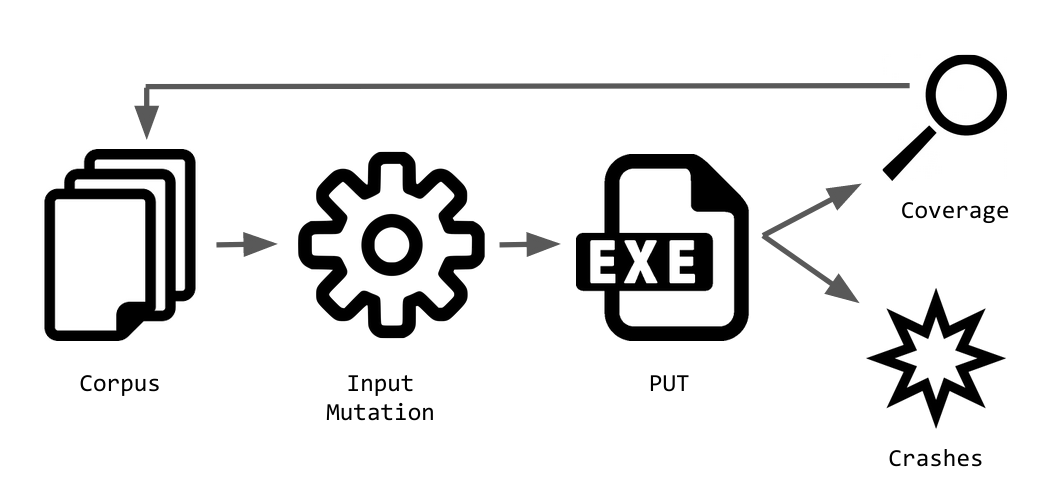
\includegraphics[scale=0.2]{img/cgf}
\centering
\caption{Basic representation of the Mutational Coverage Guided Fuzzing algorithm}
\label{fig:cfg}
\end{figure}

State of the art Coverage-Guided Fuzzers encode the approximate executed path in a representation that is easy and fast to process.
{\sc AFL++} uses a vector of 65536 entries by default, the {\it hitcounts} vector.

Each coordinate is associated with an edge and each value represents how many times the edge is executed modulo 256.

When a values greater than the previous one is registered in this vector, the fuzzer consider the input interesting and saves it.

Some extensions of CGF save also intermediate inputs that are a superset of the coverage reported in the hitcounts vector, like \cite{lafintel} \cite{ijon} \cite{besensitive}.

In general, when an input is saved, we can associate it to the testcases that generated it by mutation, the {\it parent} testcases. In this way, is easy to construct a graph of generated inputs that represents the progress of the hill climbing algorithm of the fuzzer, the {\it Generations} Graph.

% Looking for parents in this tree, we can evaluate if the intermediate inputs generated by the specific technique is effective.

\section{Methodology}

A {\em fuzzing campaign} is the process of running one or more fuzzers for a long period of time or even continously like in OSS-Fuzz \cite{serebryany2017oss}.

Security researchers tipically starts fuzzing using naive configurations and off-the-shelf fuzzers, then, meanwhile the campaign runs, observe the evolution and tune the fuzzers.

Our proposed approach aims to insert in the observation-tuning feedback loop a visual component to hekp the researcher in better understand insights about the fuzzers testing a particular target.

The data processed by {\em FuzzSplore} comes from the execution of the corpus of testcases that each fuzzer saved so far. The execution is instrumented and various properties are observed.

Then we visualize these collected properties and the user can relate them to better understand what is going. After that, the user can choose to drop some fuzzers if less effective and assign more resources (tipically CPUs) to the most effective fuzzers or tune each individual fuzzer.

The fuzzing campaing can then continue. When it saturates, the analyst can collect insights using our tool and restart the visual analytics feedback-loop.

Saturation of fuzzers, when no more additional state is explored or the number of states explodes, is a problem that was rarely addressed in academic literature but that affects each type of Feedback-driven Fuzzer \cite{saturation},  and a tool that can guide towards the selection of techniques that avoid saturation can help a lot the campaign.

\subsection{Data Retrieval}

% We developed a script to extract the data from the execution of the various instrumented programs used by each fuzzer.

We denote each fuzzer $F_i$ where $i$ is the index that identify it. 
With $PUT_i$ we denote the version of the PUT preprocessed and istrumented in order to be used by $F_i$.
$PUT_e$ is the version of the PUT that logs the edge coverage using the hitcounts vector. It has to be provided independently if it is used or not by some fuzzer $F_i$.
With $T_i(t)$ we denote the set of the saved testcases, the queue, by $F_i$ until time $t$ (seconds).

Given $t$ as the time chosen by the user to observe the progrss of the fuzzers, the Algorithm \ref{alg:data} computes the following sets:

\begin{itemize}
\item the set $C$ of all the functions $C_i \colon Time \longrightarrow NumEdges$ that relates, for the fuzzer $F_i$, a time unit to the number of discovered edges so far;
\item the set $I$ of all the functions $I_i \colon Testcase \longrightarrow \{F_j, ...\}$ that associates, for the fuzzer $F_i$, each testcase in $T_i(t)$ to the set of fuzzers that consider the testcase as interesting;
\item the set $X$ of the sets $X_i$, that maintains, for each fuzzer, the hitcounts vectors assciated with the execution of each testcase in $T_i(t)$;
\end{itemize}

\begin{algorithm}[h]
\DontPrintSemicolon
%\KwResult{The set $C$ of all the functions $C_i \colon Time \longrightarrow NumEdges$ that associates, for the fuzzer $F_i$, a time unit to the number of discovered edges so far. The set of all the functions $I_i \colon Testcase \longrightarrow \{F_j...\}$ that associates, for the fuzzer $F_i$, each testcase of $T_i(t)$ to the set of fuzzers that consider the testcase as interesting.}

  \For {$F_i$ \textbf{ in } $Fuzzers$}{
    $V_{acc} \gets (0_0 ... 0_{65536}) $\;
    
    \For {$T$ \textbf{ in } $T_i(t)$}{
      $V \gets Execute(PUT_e, T)$\;
      $X_i \gets X_i \cup \{V\}$\;
      $V, IsInteresting \gets MergeCoverage(V_{acc}, V)$\;
      \If {$IsInteresting$}{
        $C_i(Time(T)) \gets CountNotZeros(V_i)$\;
      }
    }
    
    \For {$F_j$ \textbf{ in } $Fuzzers \setminus F_i$}{
    
     $V_{acc} \gets (0_0 ... 0_{65536}) $\;
     
      \For {$T$ \textbf{ in } $T_i(t)$}{
        $V \gets Execute(PUT_j, T)$\;
        $V_{acc}, IsInteresting \gets MergeCoverage(V_{acc}, V)$\;
        \If {$IsInteresting$}{
          $I_i(T) \gets I_i(T) \cup \{F_j\}$\;
        }
      }
    
    }
    
  }

 \Return{$C, I, X$}\;
 \caption{Compute $C$, $I$, and $X$}
 \label{alg:data}
\end{algorithm}

The next item that has to be retrieved, in addition to $C$, $I$ and $X$, is the set $G$ of all the graphs $G_i$ that describes the evolution of each $T_i(t)$, the levels graph introduced in Sec. \ref{sec:back}.

We asume that each fuzzer encode the information about the parent testcases into the metadata of each testcase. In this way, it is trivial to construct the graph just reading all the metadata in $T_i(t)$.

\subsection{Visualization}

We visualize the computed data $C$, $I$, $X$, $G$ and some other properties that can be directly collected in four different views.

You can see these views with some example data in the screenshot of our implementation, in Figure \ref{fig:full}.

A timebar is used to select $t' \in [0, t]$ to ignore data ouside the selected time range and, for instance, visualize the data related to the queue $T_I(t')$ without the need to run again Algorithm \ref{alg:data}.

\subsubsection{Testcases Scatterplot}

Each $X_i$ is a matric of $|T_i(t)|$ rows in which each row is a vector of 65536 entries.

There raw numbers are raw to visualize. To handle this problem, we reduce the dimensionality of each vector $X_{i,j}$ from 65536 to 2, in order to be easily visualized in a scatterplot.

To do that, we chosen an algorithm that optimize the conservation of local distances after the dimensionality reduction, {\em t-SNE} \cite{maaten2008visualizing}. The nature of this algorithm is randomic, it needs to process $X$ entirely in order to get new vectors that are meaningfully comparable.

We experimentally observed on a test dataset that a perplexity of 30 is good enough.

The user can select groups of nodes interactively to highlight properties in the other visualiztions.

\subsubsection{Coverage Growth Plot}

$C$ can be visualized simply using a line plot with the X axis representing the domain, the time, and the Y axis the number of edges.

When a testcase is selected in the scatterplot or in the generations graph a vertical line appears at position $x$ where $x$ is the time in which the testcase was discovered.

\subsubsection{Interesting Testcases Plot}

Ths plot is used to visualize the evolution of the fuzzing algorithm in finding new testcases. The X axis represent time in seconds, the Y axis the number of new interesting testcases saved by the fuzzer in that second.
This information is directly contained in $T_i(t)$.

Here too, when a testcase is selected in the scatterplot or in the generations graph a vertical line appears at position $x$ where $x$ is the time in which the testcase was discovered.

\subsubsection{Generations Graph}

We visualize each Generations Graph $G_i$ combined with $I$. Given a fuzzer $F_j$ from the user, we highlight in graph $G_i$ each node associated with each testcase $T$ if $F_j \in I_i(T)$. In this way, the user can know if the evolution of $T_i(t)$ associated to the fuzzer $F_i$ is compatible with the selected $F_j$.

When a testcase is selected in the scatterplot, the border of the corresponding node in the graph is highlighted. The user can select additinal nodes or deselect nodes selected from the scatterplot. The scatterplot selection is sychinized in both ways witht the graph.

\subsection{Analyst Feedback}

The insights that an analyst can retrieve in order to choose or tune the fuzzers using the visualization are, but not limited to, the following:

\begin{itemize}
\item looking just at the scatterplot, the user can select a subset of fuzzers that explore different program points if the points related to each fuzzer in the graphs are clustered;
\item looking at the scatterplot and the coverage graph, the user can select a cluster of testcases that are similar and see the ability of a fuzzer in generating similar testcases in a small range of time. A fuzzer that discovers few points at time and have them distributed for all the X axis of the coverage plot should be deprioritized;
\item looking at the coverage graph, when there is a huge increment of the number of edges, the user can see if an outlier in the scatterplot was generated. This allow to isolate interesting testcases that improves a lot the coverage;
\item selecting testcases in the graph, the user can see if the testcases are similar in the scatterplot in order to understand the ability of the mutator to generate similar or different derived inputs;
\item selecting testcases in the graph and a fuzzer to cross compare, the user can know if the coverage metric of the other fuzzer is sensitive enougth to cover the selected testcases.
\end{itemize}

%\subsection{Choosing and Tuning Fuzzers}

\section{Implementation}

We created an \textsc{html} page comprised of 4 views and a filtering panel and all the components were created using the \textsc{D3.js} library.
\subsection{Testcase Scatterplot}
 
The scatterplot has as both axis a linear scale  where the points are color coded to represent a category to help the analyst distinguish the similarity in the clusters highlighted and the presence of outliers.
By brushing over the scatterplot an update routine is called to update the other 3 view with the highlighted elements in order help in finding relations.
The user can also zoom in and out which scales appropriately both axis.
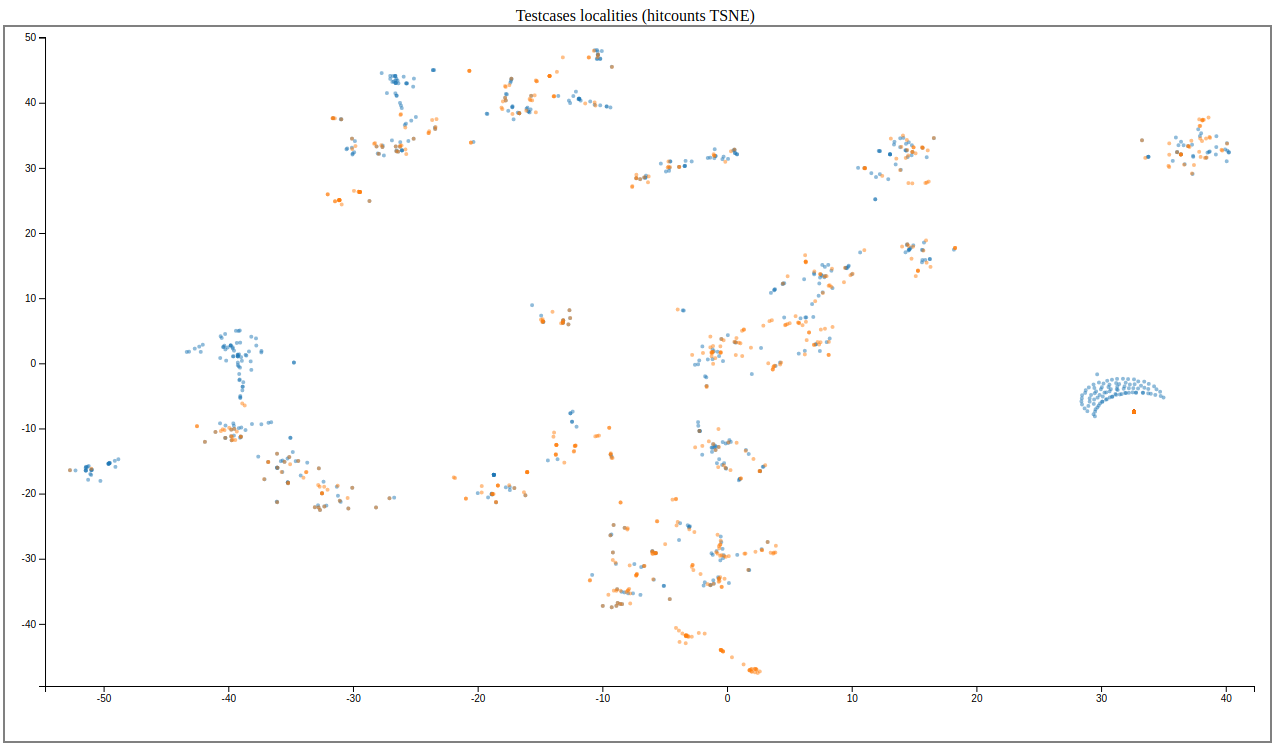
\includegraphics[scale=0.2]{img/scatterplot}

\subsection{Coverage Growth and Testcase Plots}
The Coverage graph plots the growth over time of the number of covered edges, the Testcase graph plots the nubmer of testcases over time instead, for both the bottom axis is implemented as a linear scale, for the first graph the left axis is implemented as a logarithmic scale, for the latter a linear scale is used instead.
We also implemented a zoom that keeps the lowest value pinned at the bottom and a feedback for the selected points from the coverage scatterplot or generation graph.
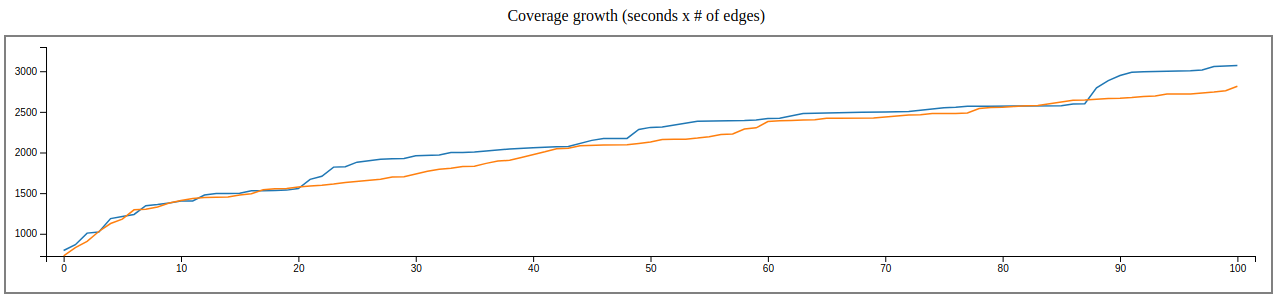
\includegraphics[scale=0.3]{img/coverage}
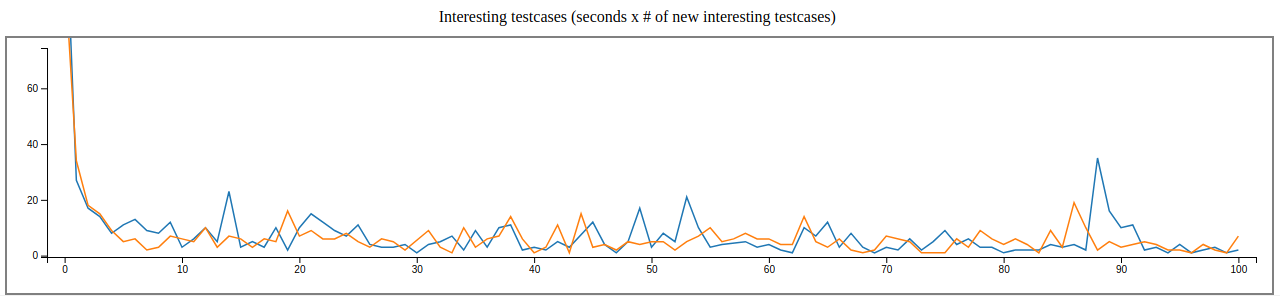
\includegraphics[scale=0.3]{img/inputs}

\subsection{Generation Graph}
The Generation Graph is created as a hierarchical layout where each data point's value is displayed as a node label. The user can zoom as well as pan over the entire view to have a better understandig of the data and when a node is selected the other graphs are updated.
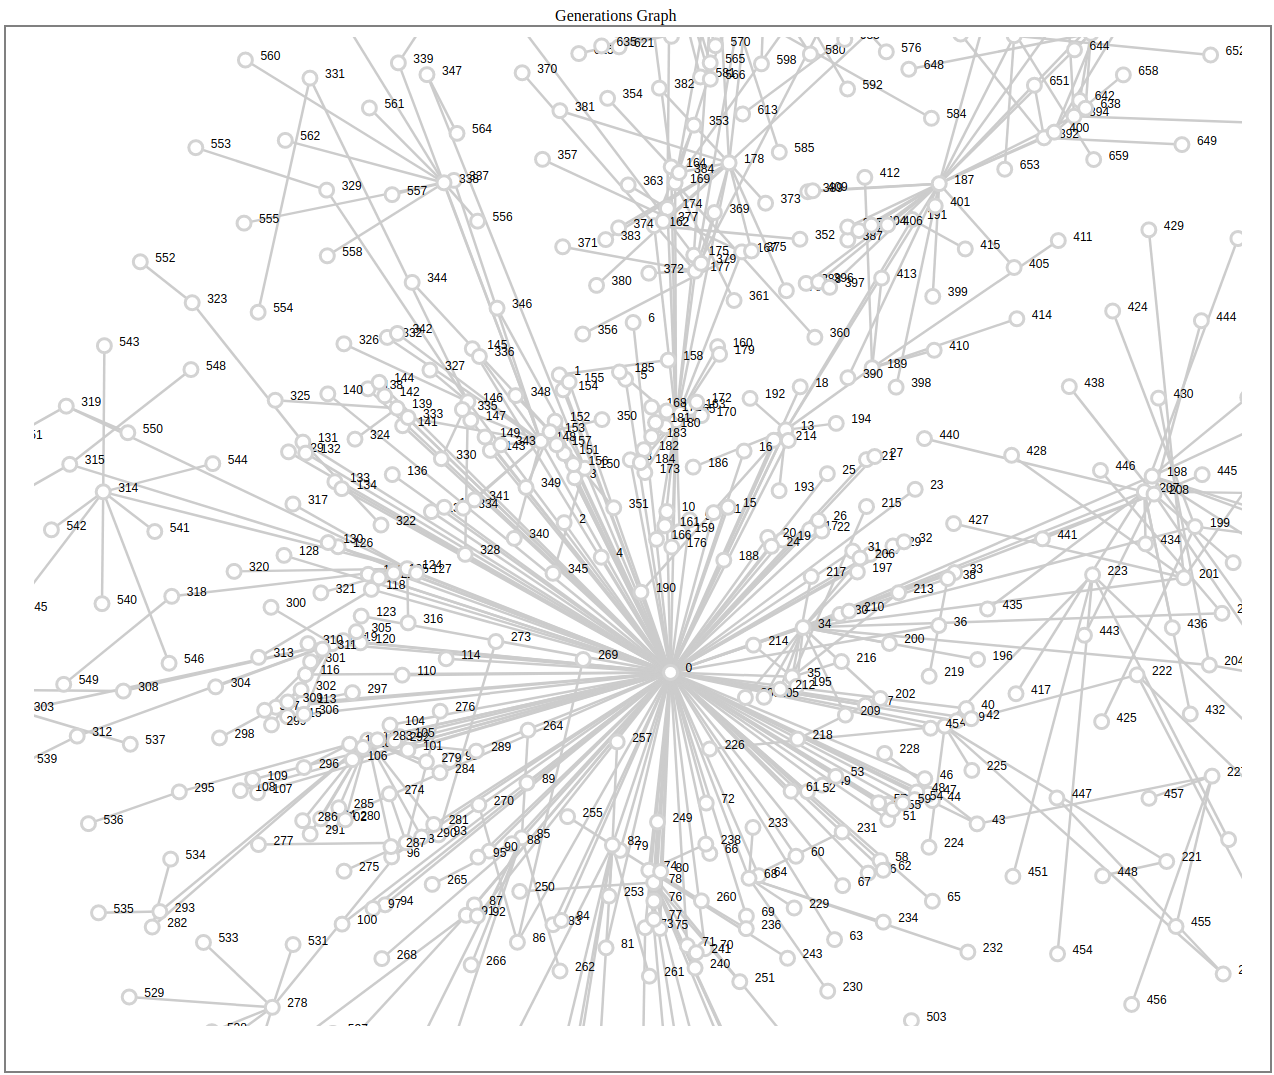
\includegraphics[scale=0.2]{img/tree}

\subsection{Filtering Panel}
The user can filter the data shown an all the 4 views by time, with a range slider located at the bottom right of the page, and by category, by clicking on the category names directly on top of the slider.
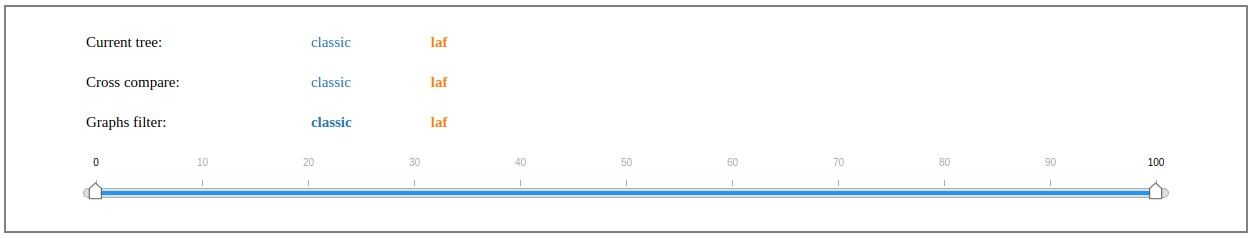
\includegraphics[scale=0.3]{img/panel}
\section{Conclusion}




\bibliographystyle{IEEEtran}
\bibliography{bibliography}

\end{document}
